\subsection{Jets}
\label{sec:jets}

Note: the jets selection has not changed with respect to the 2015 analysis. 

The jets in Run-II at CMS are reconstructed using anti-kt algorithm
with the distance parameter $D=0.4$. This was a change with respect to
the parameter distance of $D=0.5$ in Run-I due to increased pile-up in
Run-II data taking. This change resultes in smaller $\Mjj$ resolution
but induced a bias towards lower energy of the signal $\Mjj$ peak,
because less energy is clustered in a jet. This effect can be seen in
figure \ref{fig:jet-reco} of the $\Mjj$ distribution for reconstructed
jets matched to generator-level jets (that come from the Higgs) from
the Radion sample of $M=300\GeV$.

\begin{figure*}[thb]
  \centering
  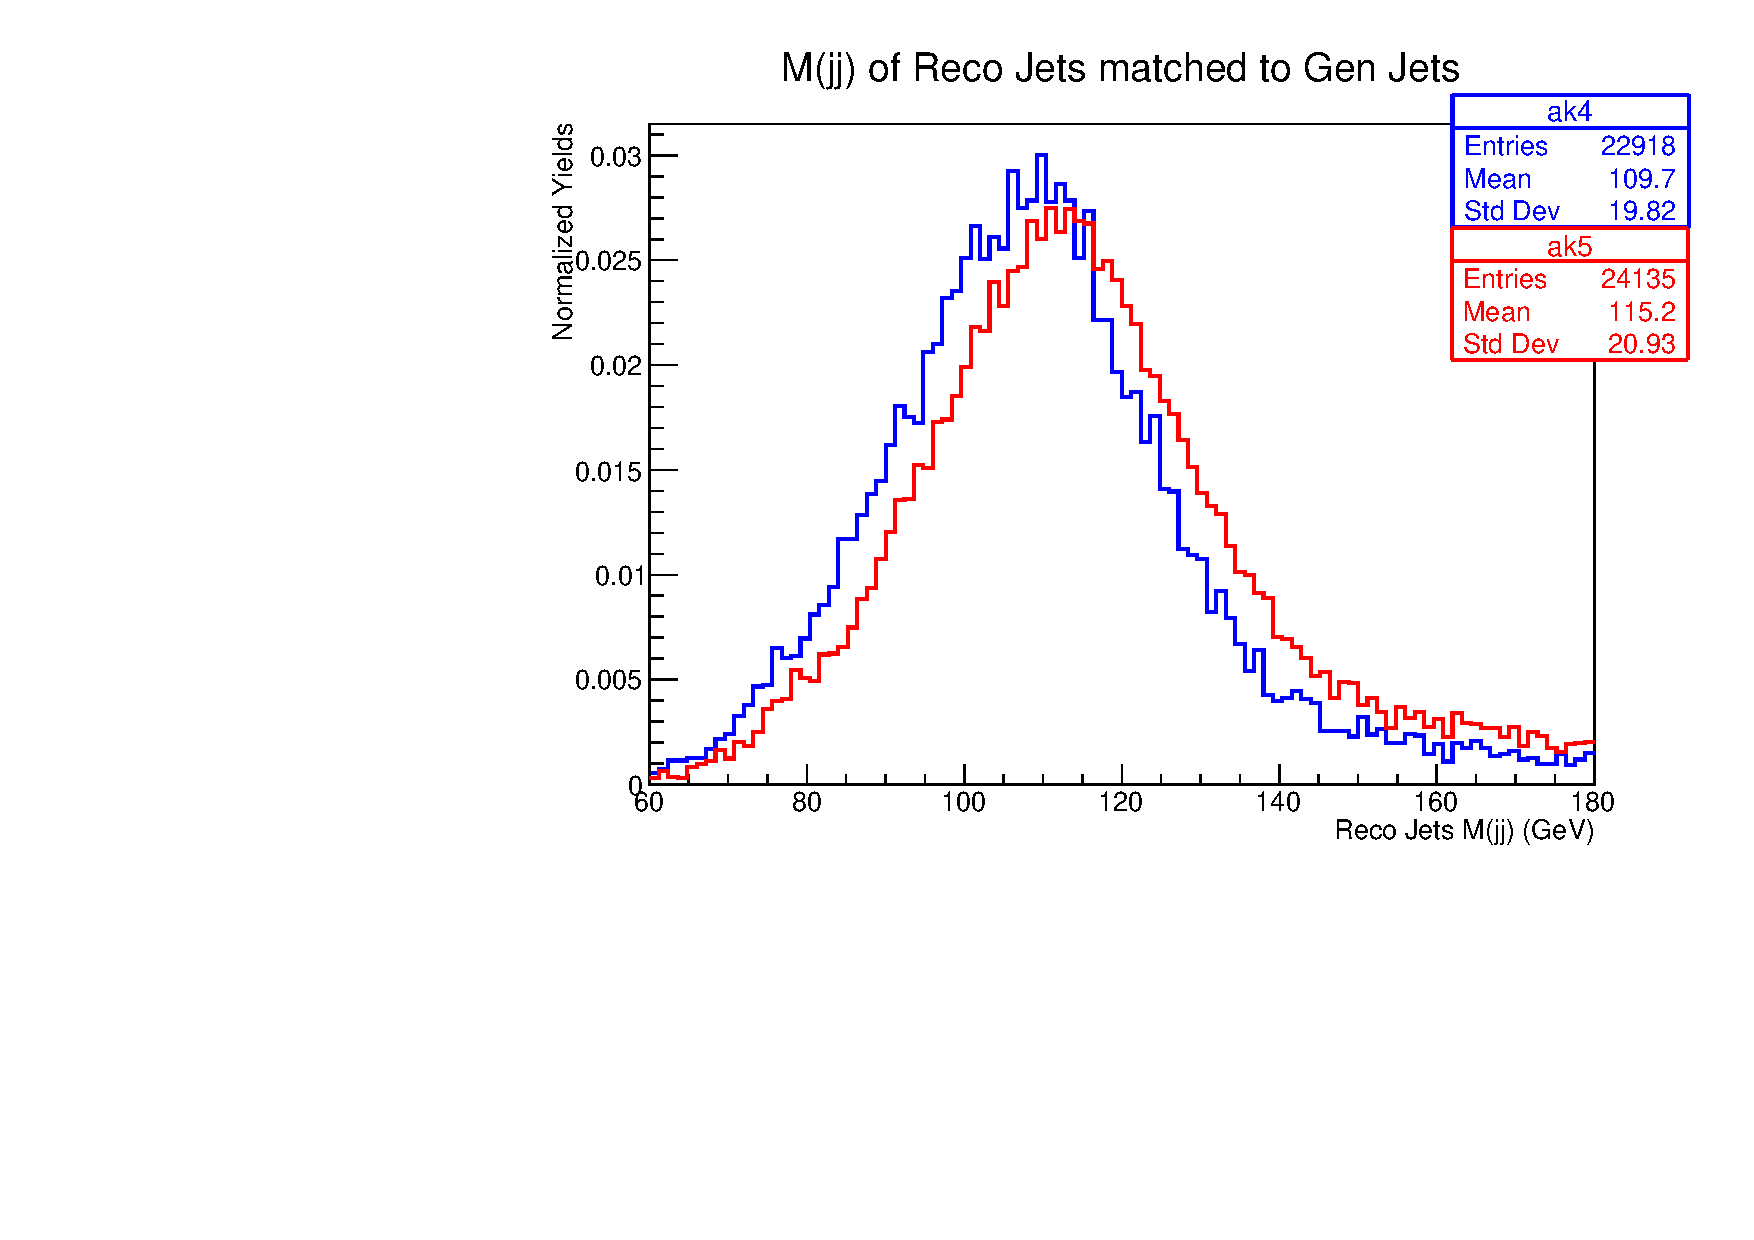
\includegraphics[width=0.45\textwidth]{figures/sec-jets/jet_rec.pdf}\hfil
  \caption{Difference between jet reconstruction used in Run I (red) and Run II (blue)}
  \label{fig:jet-reco}
\end{figure*}

We use the \textit{Loose ID} criteria to select the jets, which is described in
Ref~\cite{jetID-twiki}.

The jet candidates in the event, after passing the aforementioned ID,
must have $\PT > 25 \gev$ and $|\eta| < 2.4$ (so that they are within
the tracker of CMS and can be tagged as coming from $b$ quark). The
jets must also be outside the photon cone with a $\Delta R(j,\gamma) >
0.4$. Dijet objects are then created and only dijets with $\Mjj$ between 60 and 180 GeV 
pass the selection. If more than one dijet has passed those criteria, the dijet with two jets
with highest b-tagging score (see sec. \ref{sec:btag}) are selected as
the dijet candidate.


\subsubsection{Jet energy regression}
\label{sec:b-reg}
In addition to the misfortune of a small distance parameter of the jet
reconstruction algorithm, the energy of the jets coming from
$b$-quarks can not be fully reconstructed due to neutrinos escaping
the detector.  In order to improve the \Mjj resolution and gain in S/B
discrimination, we employ jet energy regression technique based on MC
simulated samples. We use implementation of the regression in TMVA
package and train it on $X\to\HH\to\bbbb$ MC samples. Input variables
to the training include jet kinematics, energy deposited in the
calorimeter, vertex information, and also the missing transverse
energy in the event (MET). Performance of the regression was validated
on MC signal samples as well as in data, based on $Z(\ell\ell) + bb$
events, where the \pT balance was checked of the $\pT(\ell\ell)$ and
$\pT(bb)$.  Detailed information about the training and its validation
can be found in Appendix~\ref{sec:regression}.

The effect of the regression on the analysis can be summarized in
figures \ref{fig:bregeffect}.  While data in the photon control region
remains the same, the $\Mjj$ spectrum in the signal is shifted towards
higher values (scale correction).  This leads to an improvement in the
analysis due to the gain in signal efficiency.

\begin{figure*}[thb]
  \centering
  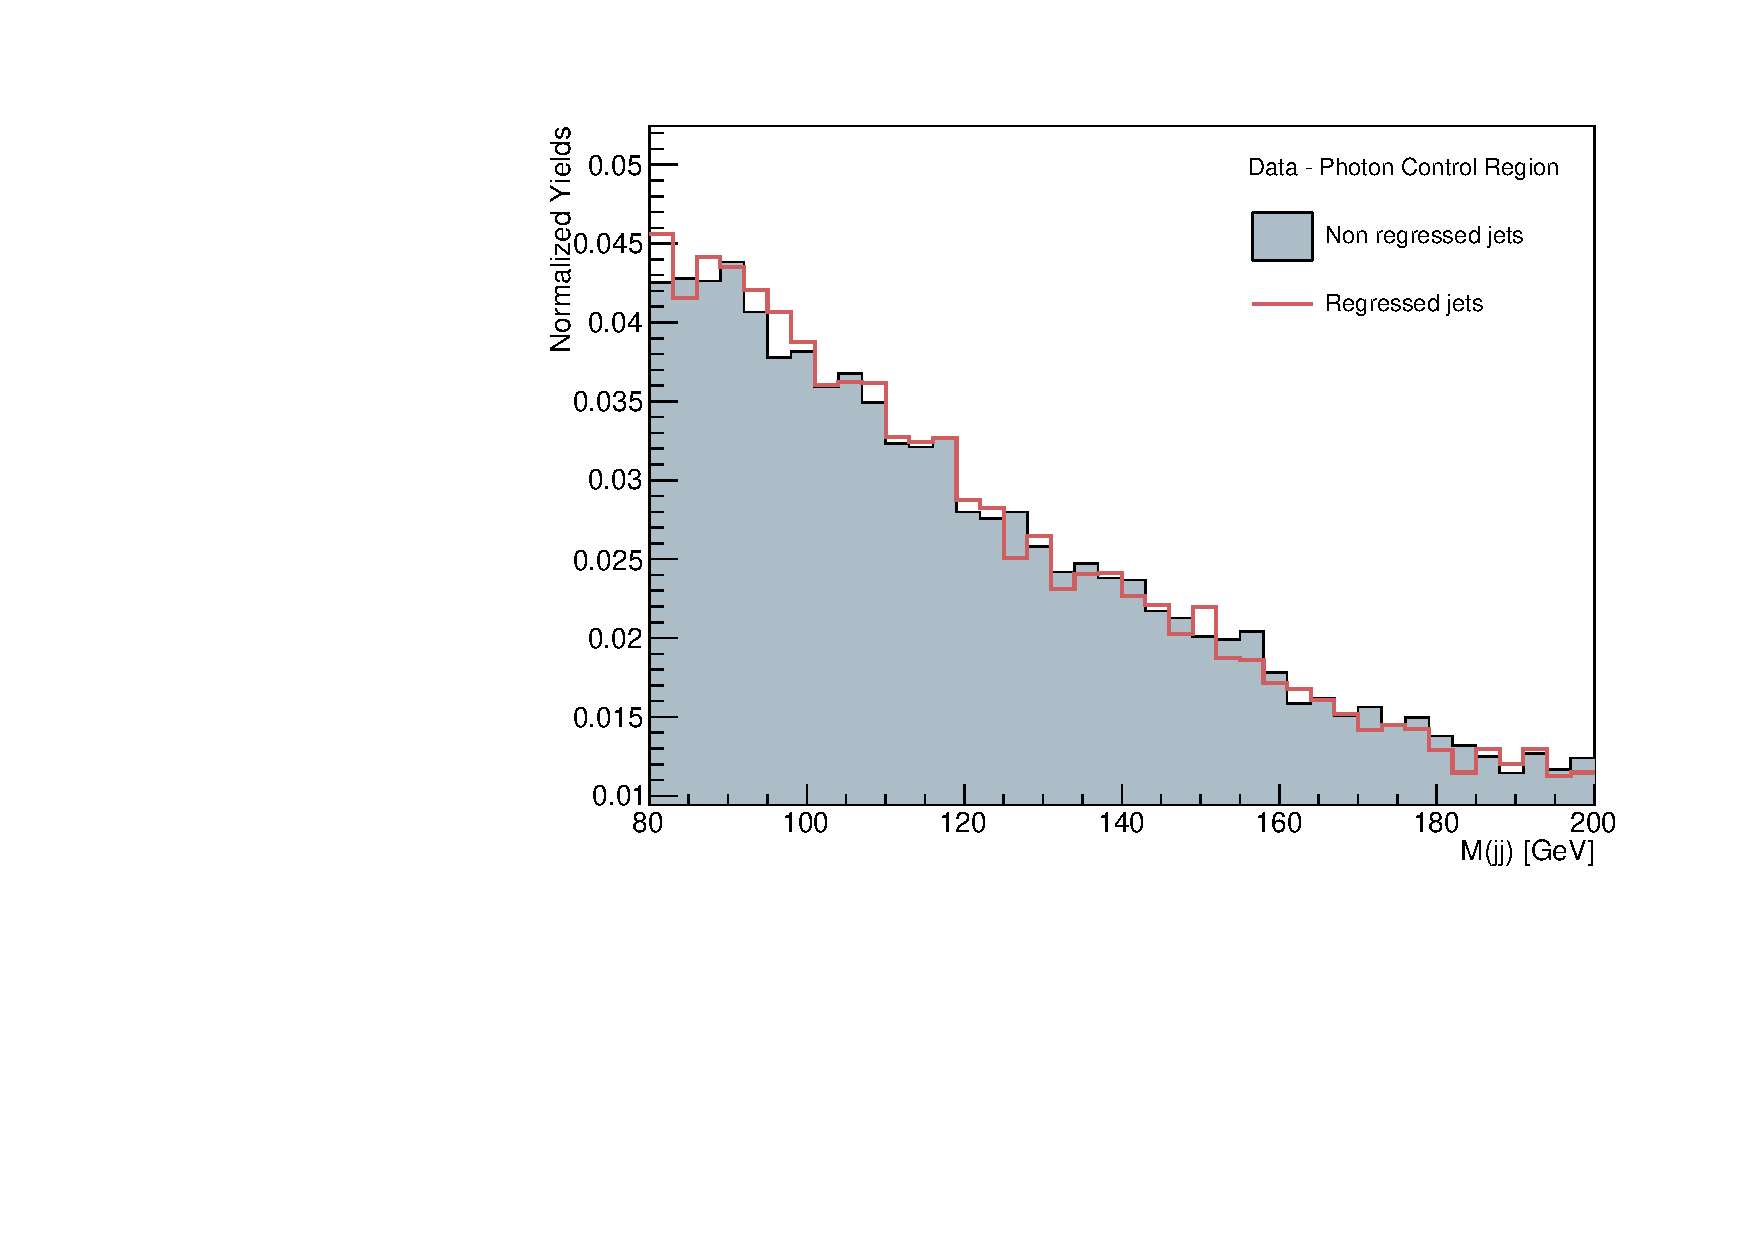
\includegraphics[width=0.45\textwidth]{figures/sec-jets/DoubleEG_dijetmass.pdf}\hfil
  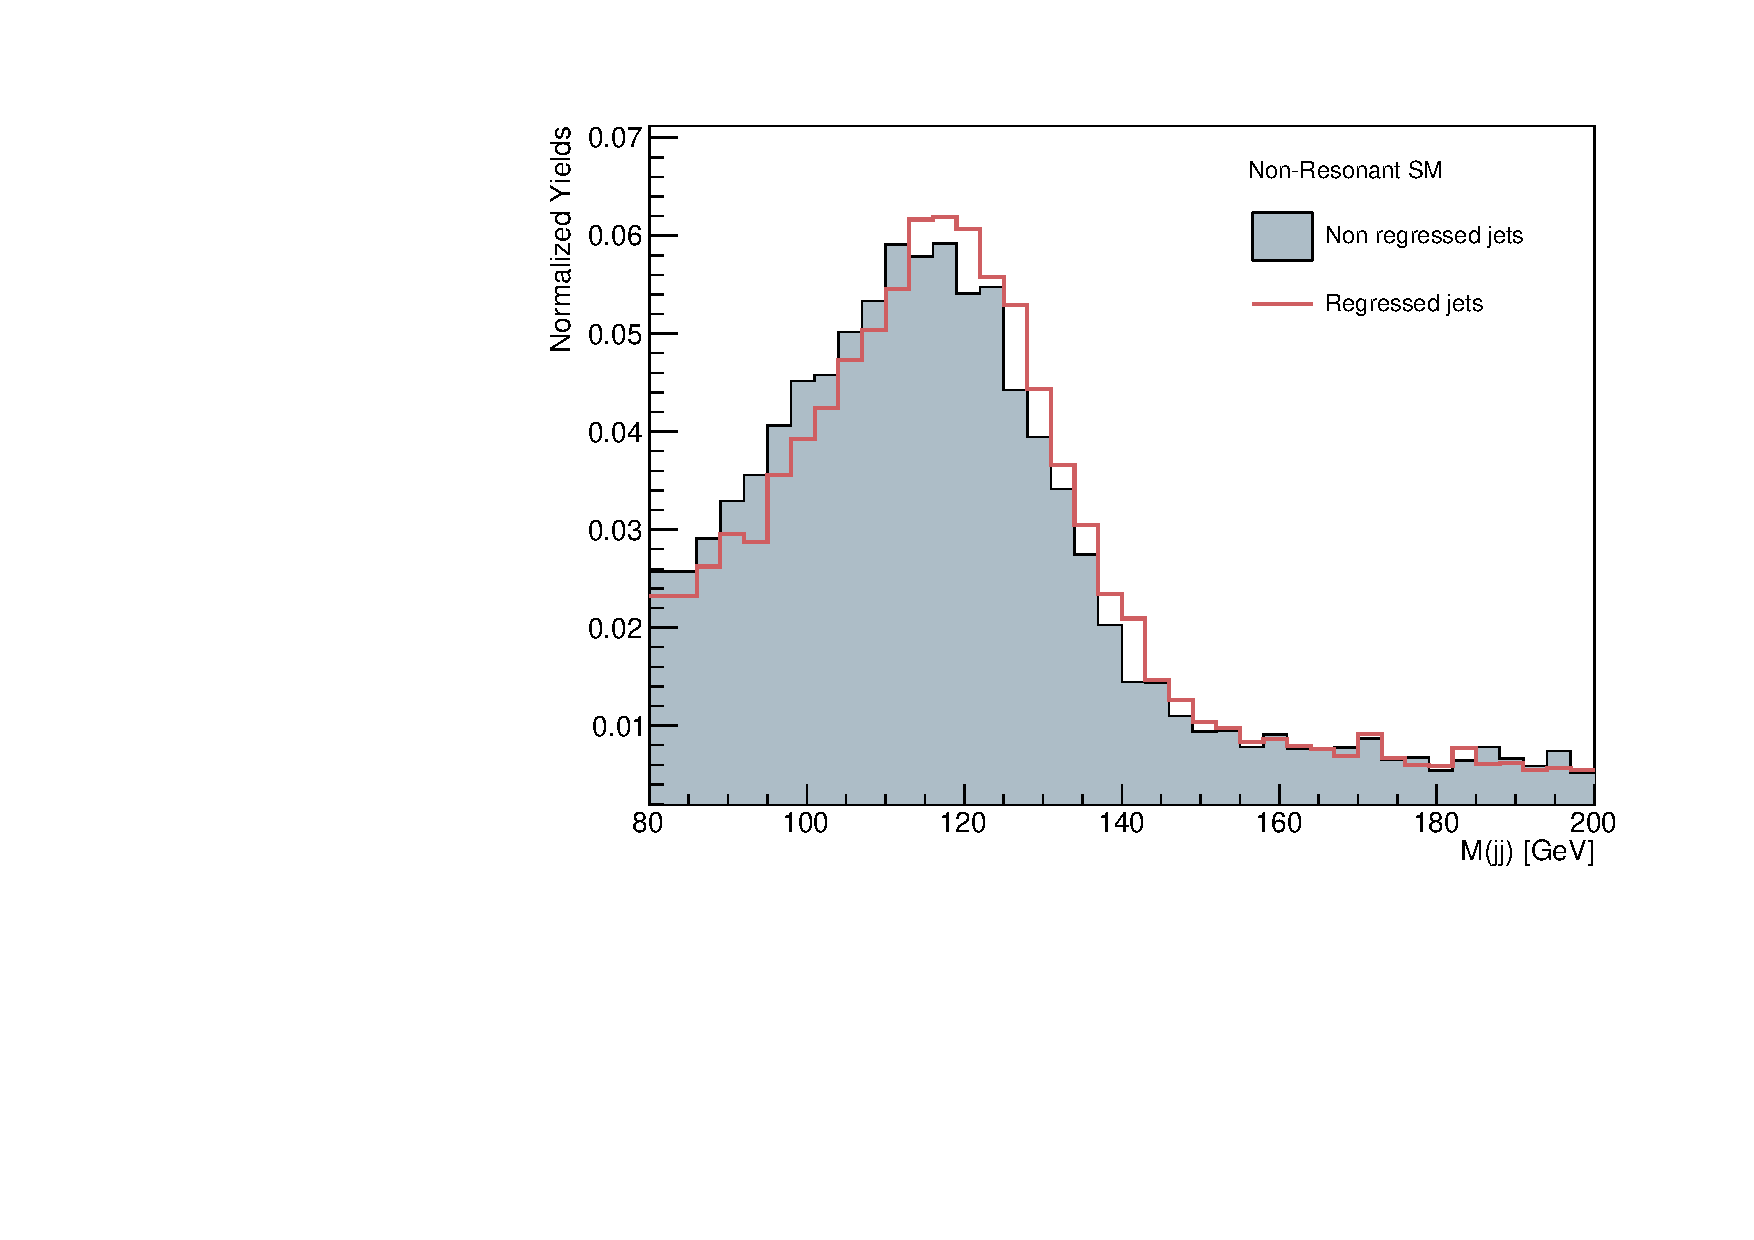
\includegraphics[width=0.45\textwidth]{figures/sec-jets/output_GluGluToHHTo2B2G_node_SM_13TeV-madgraph_dijetmass.pdf}\hfil
  \caption{Comparison between dijet invariant mass with regressed jets
    and without for data in photon control region and signal
    MC. WARNING - THESE ARE 2015 PLOTS, NEED TO UPDATE}
  \label{fig:bregeffect}
\end{figure*}



\subsubsection{B-tagging}
\label{sec:btag}

We utilize the \textit{Combined Secondary Vertex} algorithm (CSVv2) for tagging b-jets,
described in Ref.~\cite{btag-twiki}. This b-tagging score for leading and subleading jets is then used for the resonant and non-resonant analyses categorization (see section \ref{sec:cats}).

The b-tagging scale factors have been calculated according to the BTV recipe, including the in situ calculation of signal efficiency.
The signal efficiency has been calculated for all signal samples combined, in bins of $p_{T}$ and $|\eta|$.
The efficiency plots for tight WP, medium WP and loose WP can be seen in figure \ref{fig:btageff}.

\begin{figure*}[thb]
  \centering
  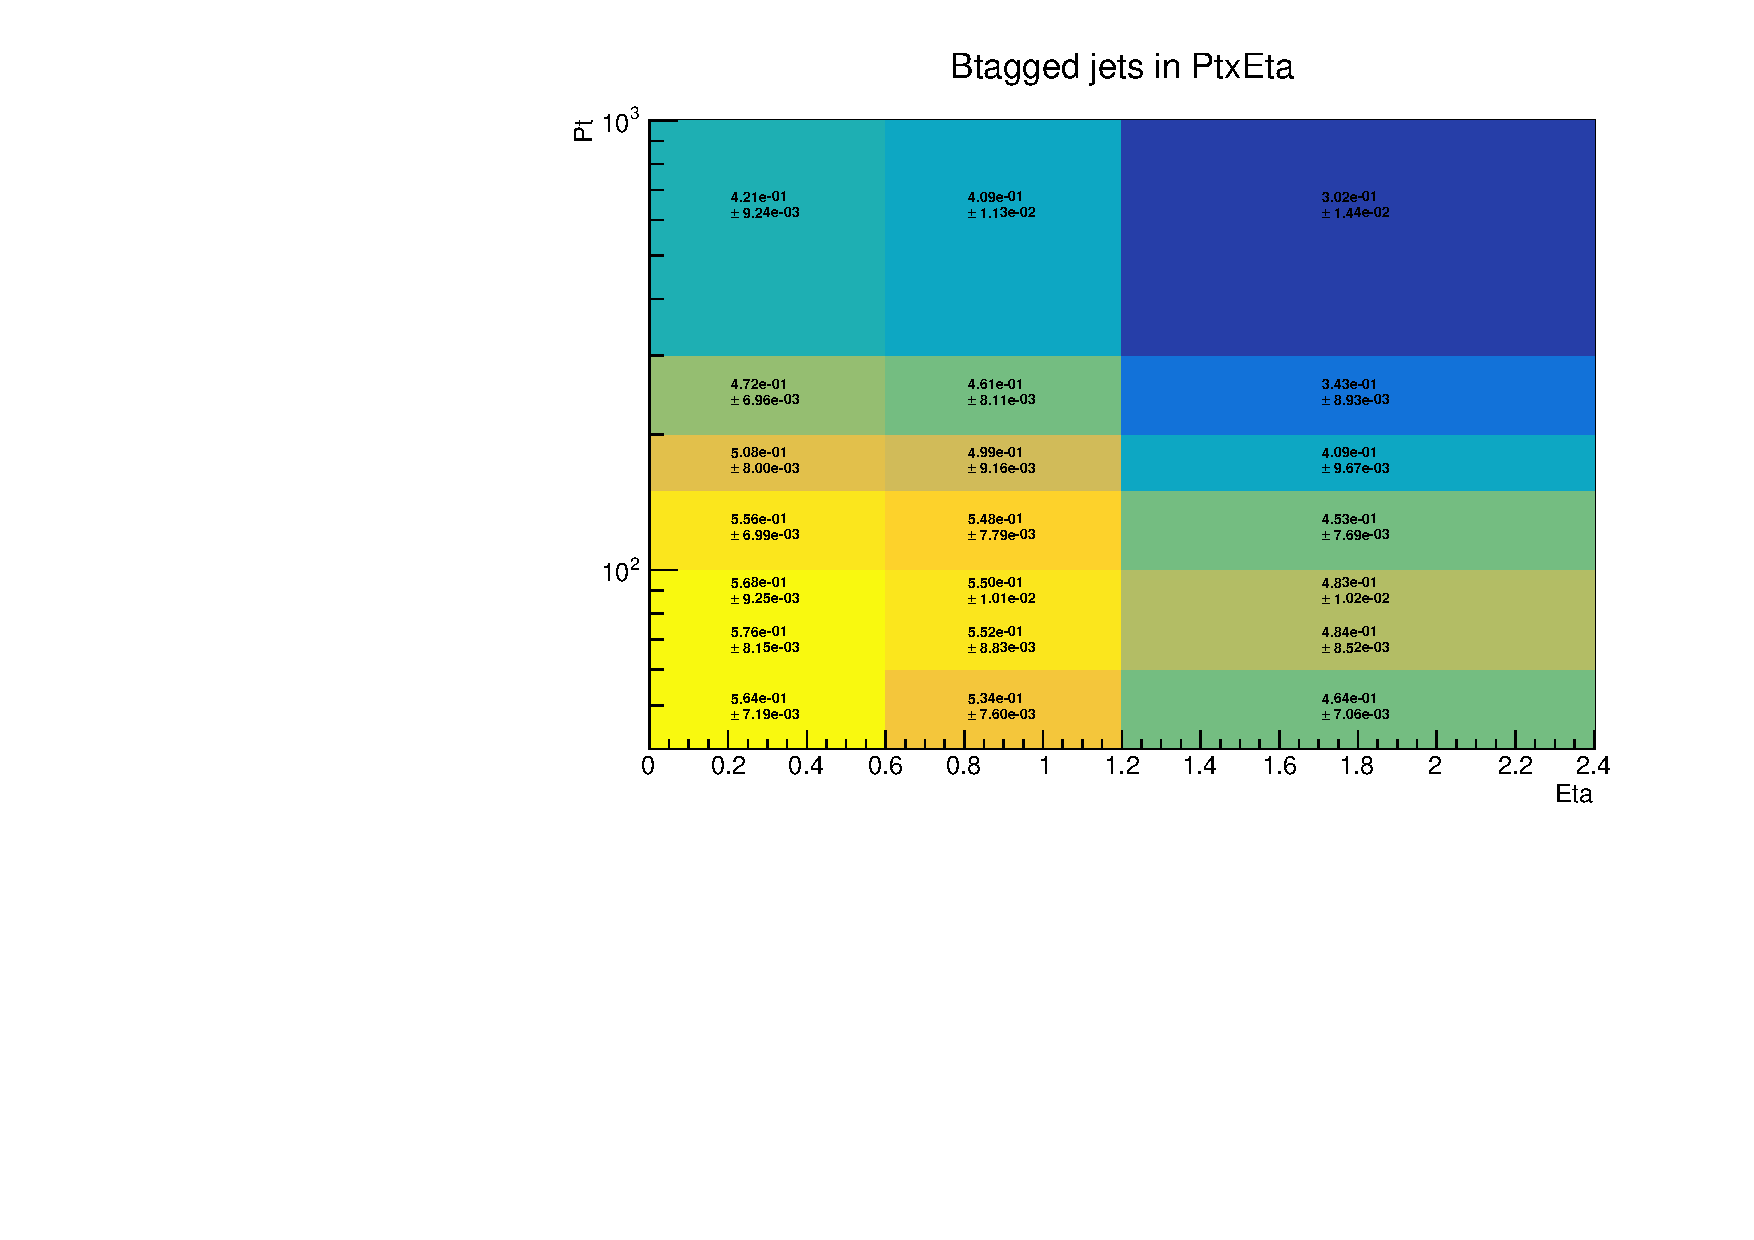
\includegraphics[width=0.45\textwidth]{figures/sec-jets/btageff_tight.pdf}\hfil
  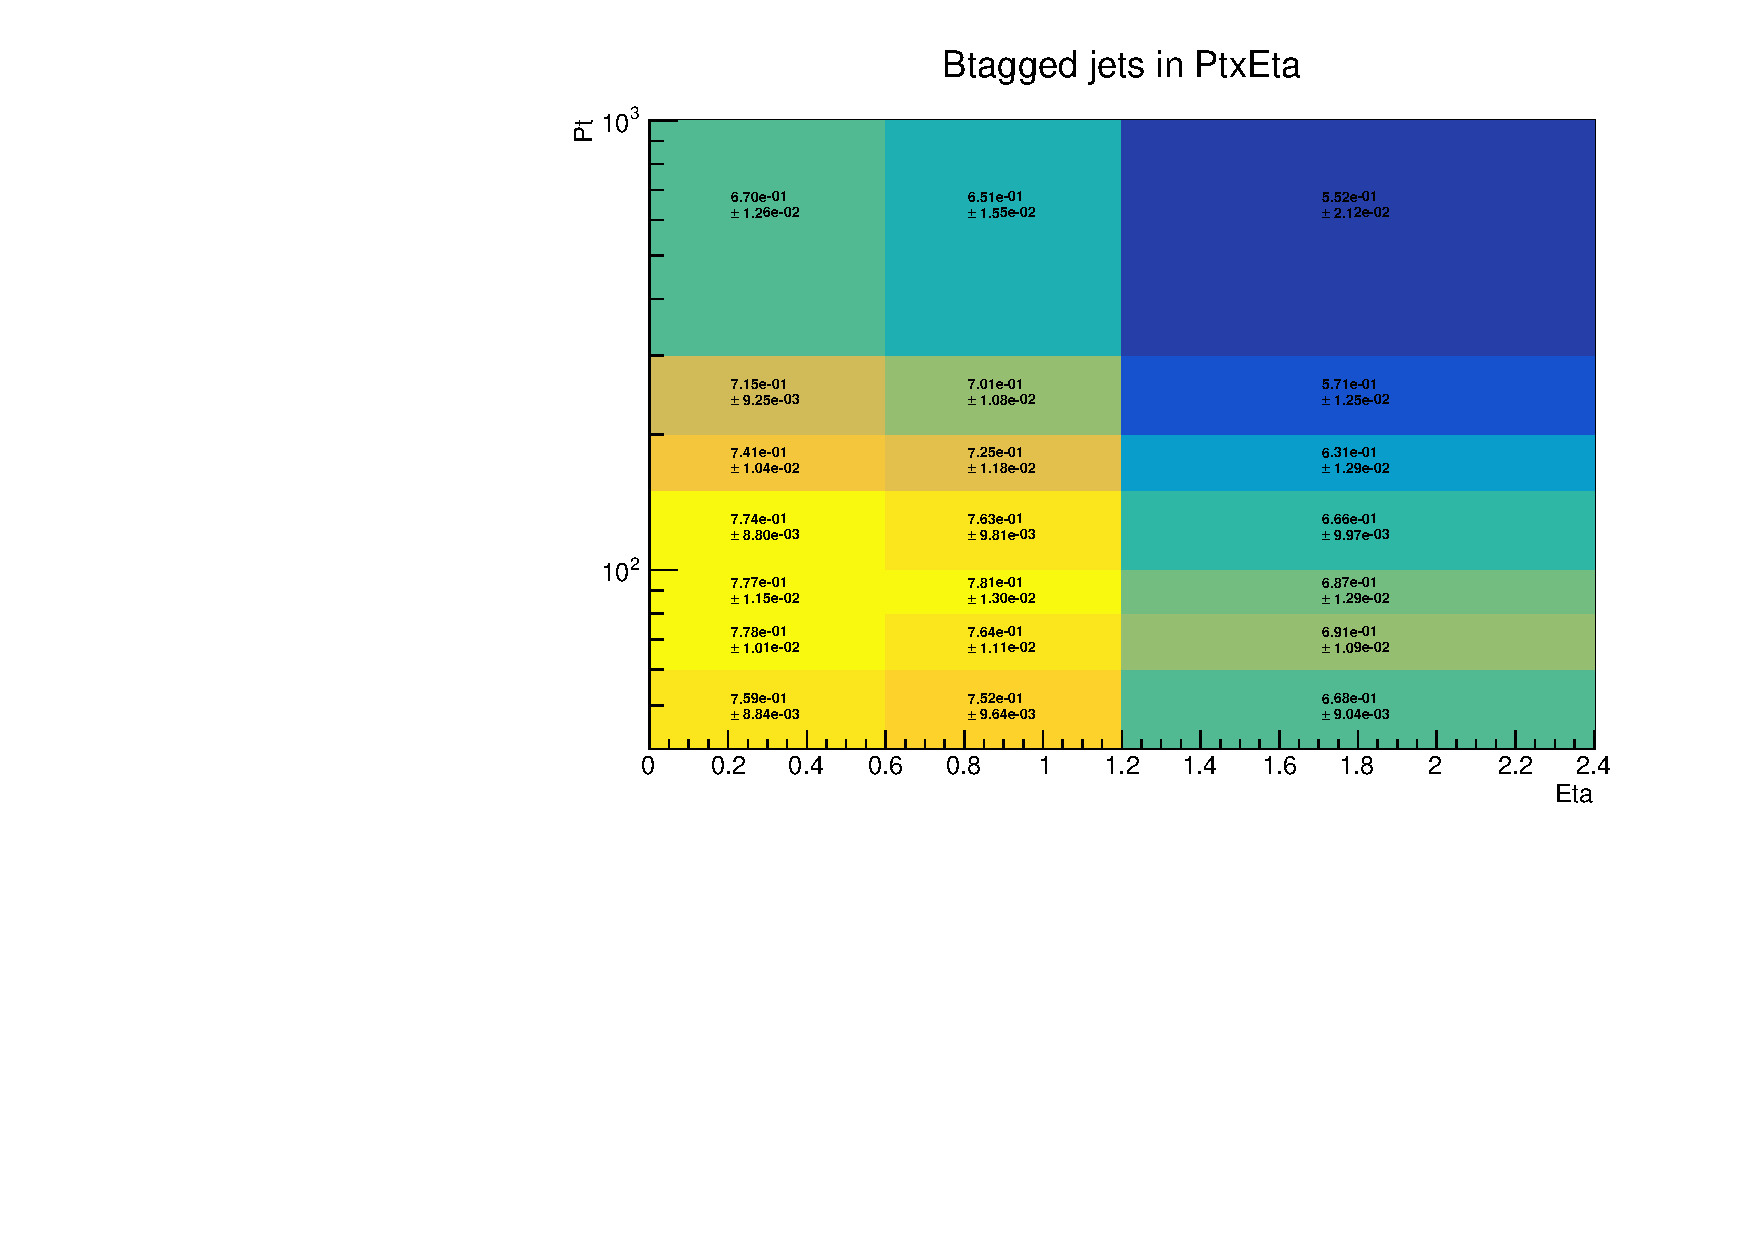
\includegraphics[width=0.45\textwidth]{figures/sec-jets/btageff_medium.pdf}\hfil
  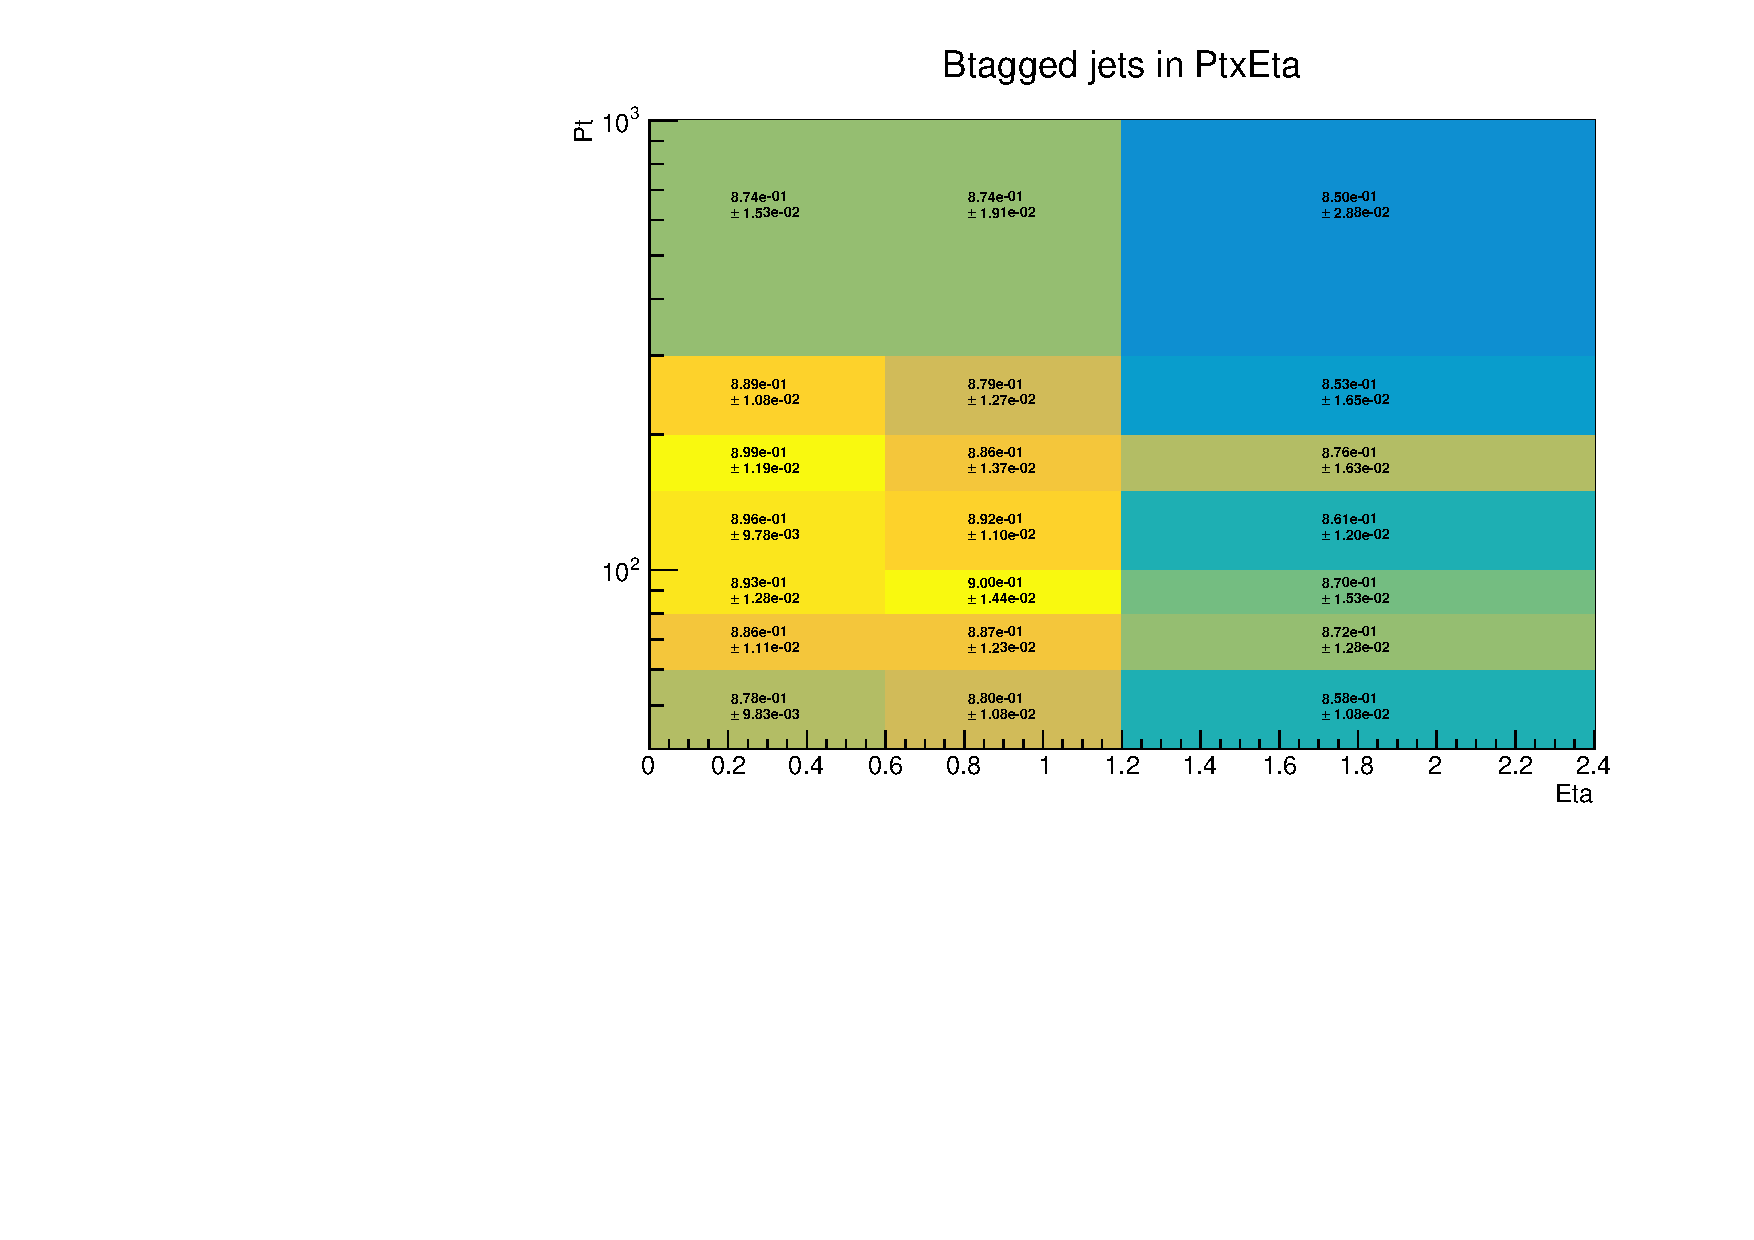
\includegraphics[width=0.45\textwidth]{figures/sec-jets/btageff_loose.pdf}\hfil 
  \caption{B-tagging efficiency for tight, medium and loose working points, as a function of jet $p_{T}$ and $|\eta|$. WARNING - THESE ARE 2015 PLOTS, NEED TO UPDATE}
  \label{fig:btageff}
\end{figure*}

